\documentclass[xcolor={usenames,dvipsnames,svgnames}, compress]{beamer}

% \usepackage[utf8]{inputenc}
\usepackage{booktabs}
\usepackage{dcolumn}
\usepackage{colortbl}

% \usepackage[style=authoryear-comp, backref=true]{biblatex}
\usepackage{ifxetex}
\usepackage{amsmath}
\usepackage{biblatex}
% 
\usepackage[no-math]{fontspec}

%
% CLIPS listings
%\usepackage[utf8]{inputenc}
\usepackage{listings}
\usepackage{xcolor}


%
% I asked on stackoverflow for rainbow parentheses
% http://tex.stackexchange.com/questions/235740/rainbow-parentheses-in-lisp-listings
% the palette is from solarized theme
\definecolor{solarized-cyan}{RGB}{42, 161, 152}
\definecolor{solarized-magenta}{RGB}{211, 54, 130}
\definecolor{solarized-yellow}{RGB}{181, 137, 0}
\definecolor{solarized-violet}{RGB}{108, 113, 196}
\definecolor{solarized-red}{RGB}{220, 50, 47}
\definecolor{solarized-orange}{RGB}{203, 75, 22}
\definecolor{solarized-grey}{RGB}{101, 123, 131}

\lstdefinelanguage{clips}
{
  classoffset=0,
  morekeywords ={deffunction, deftemplate, defglobal, defmodule, defrule, deffacts, nil, assert, retract},
  keywordstyle=\bfseries\color{solarized-orange},
  classoffset=1,
  morekeywords ={delcare, salience, run, slot, multislot, clear, reset, facts, exit, agenda, initial-fact, watch, ppdefrule, unwatch, printout, if, then, else, while, loop-count, crlf, read, readline},
  keywordstyle=\bfseries,
  %classoffset=2,
  %keywordsprefix=\?,
  %alsoletter=\?,
  %keywordstyle=\itshape\color{solarized-red},
  classoffset=0,
  sensitive=true,
  morecomment=[l]{;},
  morestring=[b]{"},
  stringstyle=\color{solarized-grey},
  basicstyle=\scriptsize,%\ttfamily\scriptsize,
  numbers=left,
  numbersep=-5pt,
  numberstyle=\tiny,
  showstringspaces=false,
  }

\renewcommand{\ttdefault}{pcr}

% egreg's modulo macro (see http://tex.stackexchange.com/a/34449/21891)
\def\truncdiv#1#2{((#1-(#2-1)/2)/#2)}
\def\moduloop#1#2{(#1-\truncdiv{#1}{#2}*#2)}
\def\modulo#1#2{\number\numexpr\moduloop{#1}{#2}\relax}    

\makeatletter

% a TeX counter to keep track of the nesting level
\newcount\netParensCount@clisp

% Modify how ( and ) get typeset depending on the value of the counter
% (Based on Ulrike Fischer's approach to modifying characters in listings;
% see http://tex.stackexchange.com/a/231927/21891)
\lst@CCPutMacro
\lst@ProcessOther{`(}{{%
    \ifnum\lst@mode=\lst@Pmode\relax%
    \rainbow@clisp{(}%
    \global\advance\netParensCount@clisp by \@ne%
    \else
    (%
    \fi
  }}%
\lst@ProcessOther{`)}{{%
    \ifnum\lst@mode=\lst@Pmode\relax%
    \global\advance\netParensCount@clisp by \m@ne%
    \rainbow@clisp{)}%
    \else
    )%
    \fi
  }}%
\@empty\z@\@empty
% Color its argument based on the value of the \netParensCount@clisp counter
% (modulo 5)
\newcommand\rainbow@clisp[1]{%
  \ifcase\modulo\netParensCount@clisp 5\relax%
  \textcolor{solarized-cyan}{\bfseries#1}%
  \or
  \textcolor{solarized-yellow}{\bfseries#1}%
  \or
  \textcolor{solarized-magenta}{\bfseries#1}%
  \or
  \textcolor{solarized-violet}{\bfseries#1}%
  \else
  \textcolor{solarized-red}{\bfseries#1}%
  \fi
}

% Alternatively, you could simplify the definition of \rainbow@clisp to...
% \newcommand\rainbow@clisp[1]{%
% \textcolor{color\modulo\netParensCount@clisp 5}{#1}%
% }
%   ... but this assumes that the colours have names of the form color<i>,
%   where <i> is a positive integer

%   reset the counter at the beginning of each listing
%   (just in case there were unmatched parentheses in a previous listing)
\lst@AddToHook{PreInit}{%
  \global\netParensCount@clisp 0\relax%
}

\makeatother




\lstnewenvironment{clips-code}[1][]
{\lstset{language=clips,
    #1
  }}
{}






%%% Local Variables:
%%% mode: latex
%%% TeX-master: t
%%% End:


\definecolor{jess-fucsia}{RGB}{170, 0, 127}
\definecolor{violent-green}{RGB}{0, 128, 96}
\definecolor{ny-orange}{RGB}{255, 128, 0}

\hypersetup{
  colorlinks=true,       % false: boxed links; true: colored links
  linkcolor=jess-fucsia,          % color of internal links (change box color with linkbordercolor)
  % citecolor=green,        % color of links to bibliography
  %filecolor=magenta,      % color of file links
  urlcolor=jess-fucsia           % color of external links
}

%%% Local Variables:
%%% mode: latex
%%% TeX-master: t
%%% End:



\usetheme{enziteto}

\setbeamertemplate{headline}{}

%%%%%%%%%%%%%%%%%%%%%%%%%%%%%%%%%%%%%%%%%%%%%%%%%%%%%%%%%%%% 
%%%%%%%%%%%%%%%%%%%%%%%%%%%%%%%%%%%%%%%%%%%%%%%%%%%%%%%%%%%% 
%%%%%%%%%%%%%%%%%%%%%%%%%%%%%%%%%%%%%%%%%%%%%%%%%%%%%%%%%%%% 


\begin{document}

\title{CLIPS: Facts, Rules, Inference}
\author{Antonio Vergari}
% \institute{Lacam$@$DIB$@$Uniba}
\institute{Università degli Studi di Bari}
\department{Dipartimento di Informatica}
\laboratory{LACAM}
\group{Machine Learning}
\institutelogo{
\includegraphics[width=25pt]{Figures/unibaba}}
\lablogo{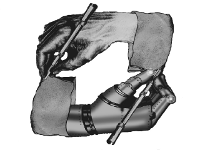
\includegraphics[width=35pt]{Figures/lacam}}

\footnotesize \let\small\footnotesize

{
  \setbeamertemplate{headline}{}
  \setbeamertemplate{footline}{}
  \begin{frame}
    \titlepage
  \end{frame}
}



\begin{frame}
  \frametitle{A first example}
  \framesubtitle{With a family DAG}
  This is our first take on a very simple \textbf{conceptualization}
  task.\par
  Suppose we want to represent the relationships in a family as
  sketched in this dag.\par
  The basic info we get are the persons' names,
  their \emph{gender} (names in italics stand for women) and their \emph{parenthood}
  (edges).
  \begin{center}
    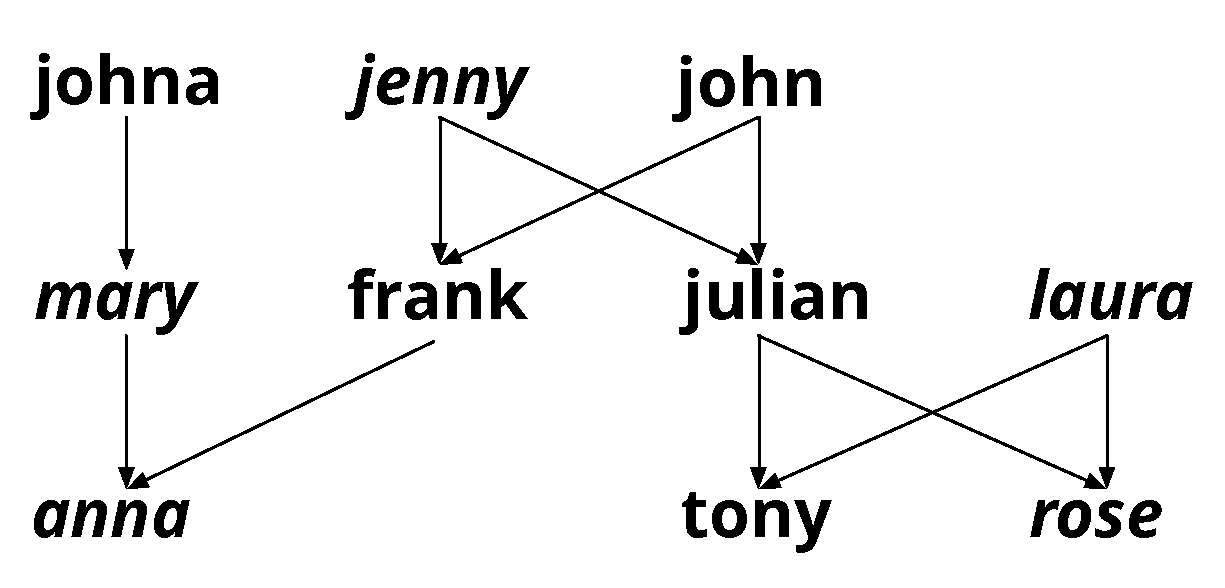
\includegraphics[width=0.7\textwidth]{Figures/family_dag}
  \end{center}
  
  
\end{frame}

\begin{frame}[fragile,fragile,fragile,fragile]
  \frametitle{family DAG I}
  \framesubtitle{Facts and rules}
  We can use \emph{\textbf{facts}} to represent what we know about this small
  world.
{\color{violent-green}\begin{verbatim}
Julian is a male. Laura is a female.
Tony is a male. Rose is a female.
 ...
Julian is Tony's parent. Laura is Tony's parent.
\end{verbatim}}
  What if now we'd like to assert something about uncle-nephew
  relationships?
{\color{violent-green}\begin{verbatim}
Frank is Tony's uncle.
\end{verbatim}}
  We can introduce \emph{\textbf{rules}} to represent how to automatically derive new
  facts, i.e. new knowledge.
{\color{ny-orange}\begin{verbatim}
IF X is Y's brother AND Z's father, THEN Y is Z's uncle.
\end{verbatim}}
  but we need to specify what brother and father mean in the first
  place... 
\end{frame}

\begin{frame}[fragile,fragile]
  \frametitle{family DAG II}
  \framesubtitle{more rules}
  
  A generic rule to derive fathers' names is straightforward:
  {\color{ny-orange}\begin{verbatim}
IF X is male AND X is Y's parent, THEN X is Y's father.
\end{verbatim}}
  
  To derive what a brother is we need to introduce one more variable
  and 
  {\color{ny-orange}\begin{verbatim}
IF X is Y's parent AND X is Z's parent AND Z is male,
THEN Z is Y's brother.
\end{verbatim}}
  
  
  Pretty simple indeed.\par\bigskip
  
  Problems: how to formalize this in CLIPS? how to let CLIPS
  infer new knowledge?\par\bigskip
  
  We will dive a bit into CLIPS logics and syntax before answering to it.
  
\end{frame}

\begin{frame}[fragile]
  \frametitle{family DAG in CLIPS}

  A simple implementation in CLIPS of a portion of the KB and the father
  inference rule. This may appear scary\dots
  \begin{clips-code}
    (deffacts family-dag
        (parent julian tony)
        (parent julian rose)
        (parent laura tony)
        (parent laura rose)
        (male tony)
        (male julian)
        (female rose))
        
    (defrule fatherhood
    "match-and-assert all father-child relationships"
        (male ?father)
        (parent ?father ?child)
        =>
        (assert (father ?father ?child))
        (printout t ?father " is " ?child "'s father "))
        
  \end{clips-code}\footnotenomarkleft{A typographical note: keywords
    are in bold, construct defining keywords are also orange. Nested
    parentheses are rainbow colored as in \href{http://www.emacswiki.org/emacs/RainbowDelimiters}{\textsf{emacs
        rainbow-delim-mode}} for the sake of legibility.}
\end{frame}

\begin{frame}[fragile]
  \frametitle{CLIPS}
  \framesubtitle{A LISPy functional programming foretaste}
  \begin{clips-code}[numbers=none]
    ; this is a comment in CLIPS
  \end{clips-code}
  Logical blocks and function calls are delimited by parentheses.\par
  Mind the \emph{prefix notation} for operators.
  \begin{clips-code}[numbers=none]
    (+ 2 3)
  \end{clips-code}
  
  Functional composition is achieved by nesting parentheses, \href{http://c2.com/cgi/wiki?LostInaSeaofParentheses}{at any
  level}. 
  \begin{clips-code}[numbers=none]
    (+ (* (* 3 (/ 1 3)) (/ 5 (+ 4 1))) 0)
  \end{clips-code}
  In truth, a pair of parentheses identifies a list.\par
  The first element of a list is a function identifier, the others are
  the function operands.\par
  
  \begin{clips-code}[numbers=none]
    (+ 2 3 4 5 6) ;; lists of arguments => variadic functions
  \end{clips-code}

  We will return to functional programming aspects later; for the time
  being, just pay attention to syntax error and evaluation order:
  \begin{clips-code}[numbers=none]
    (printout t "Beware order" (read) crlf)
  \end{clips-code}
\end{frame}

\begin{frame}[fragile]
  \frametitle{Command-line REPL}
  
  The command-line version of CLIPS lets you write instructions into
  it (mind nested parentheses and line breaks if you do not want syntax errors).
  \begin{clips-code}[numbers=none]
    CLIPS> (+ 2 3)
    5 ;; if it can be evaluated it is printed on stdout
    clisp> (printout t "Beware order" (read) crlf)
    Beware order  5
    5
    CLIPS> (exit) ;; ending the interpreter
  \end{clips-code}\bigskip
  
  Like many other interpreted languages, the main interaction happens through a \textsf{R}ead-\textsf{E}val-\textsf{P}rint
  \textsf{L}oop.
  \begin{clips-code}[numbers=none]
    (loop (print (eval (read)))) ;; this is LISP, not CLIPS!
  \end{clips-code}
  
 % \begin{clips-code}
  %   (deffunction
  %   (a b)
  %   ``''
  %   (if (a)
  %   then (b)))
  % \end{clips-code}
  
\end{frame}

\begin{frame}[fragile]
  \frametitle{Some handy functions}
  \begin{minipage}[t]{0.45\linewidth}
    \begin{clips-code}[numbers=none]
      ;; math functions
      (+ 2 4) ; 6
      (* 2 4) ; 8
      (** 2 4) ; 16.0
      (log10 100) ; 2.0
      (div 33 2 3 5) ; 1
      (max 3 9.0 -2) ; 9.0
      (abs -2.0) ; 2.0
      (float 33) ; 33.0
      (integer 4.2) ; 4
      (round 3.7) ; 4
      (cos 0) ; 1
      (pi) ; 3.14159...
      ;; logical ops
      (> 1 0) ; TRUE
      (and TRUE FALSE) ; FALSE
    \end{clips-code}
  \end{minipage}
  \begin{minipage}[t]{0.45\linewidth}
    \begin{clips-code}[numbers=none]
      ;; std I/O
      (read) ; reads a symbol
      (readline) ; reads a line
      (get-char t) ; reads a char
      (format t "like in %s\n" C)
      (printout t
          "This is a string" crlf)
      ;; file I/O
      (open example.txt
          file-stream "w")
      (printout file-stream
          "capercaillie" crlf)
      (close file-stream)
      (open example.txt
          file-stream)
      (get-char file-stream)
    \end{clips-code}
  \end{minipage}
\end{frame}

\begin{frame}
  \frametitle{GUI IDE}
  For some platforms\footnote{For GNU/Linux distros there should be an old,
    unmantained, package called \textsf{xclips}. If you manage to get
    it to work.} you can use a little IDE that offers a console
  and some windows to inspect the working memory, the agenda, object
  instances and the build constructs.
  \begin{center}
    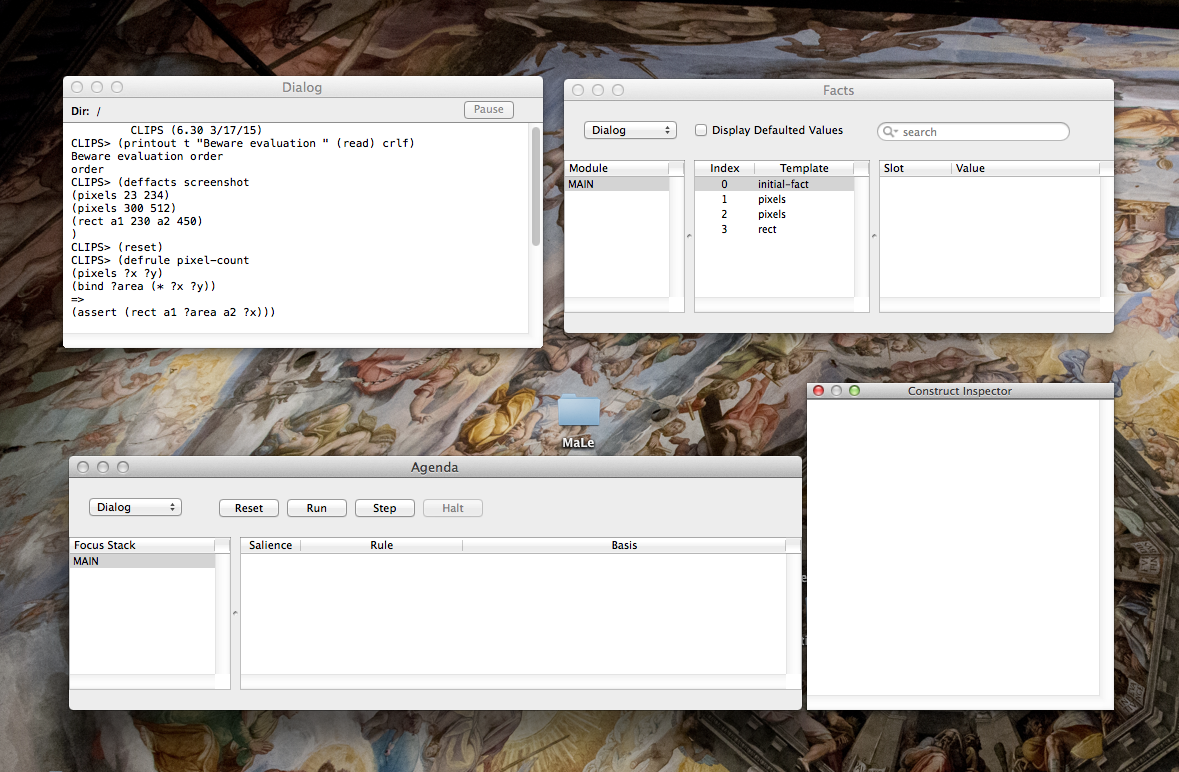
\includegraphics[width=0.7\textwidth]{Figures/clips-IDE}
  \end{center}
  
  
\end{frame}

\section{Facts}
{\setbeamertemplate{headline}{}
  \begin{frame}
    \sectionpage
  \end{frame}
}

\begin{frame}
  \frametitle{Some facts about facts (a reminder)}
  A fact is a piece of information we know about the world that we can represent, and on which we
  can base our inference.\par\bigskip
  
  An \textbf{\emph{asserted}} fact defines something that is true in our \emph{current} state
  of the world.\par\bigskip
  
  The \emph{\textbf{Working Memory}} (WM) is the current collection of
  all asserted facts. Additional facts can be added to the WM
  (\emph{asserted}), removed (\emph{retracted}) and
  modified.\par\bigskip

  CLIPS implements the \textbf{\emph{RETE}} algorithm and its data
  structure: the WM is modelled as a network of patterns efficiently
  matching the asserted facts. 
  
\end{frame}

\begin{frame}[fragile]
  \frametitle{Ordered Facts}

  Facts can be defined by a \emph{name} and a list of properties.
  \begin{clips-code}[numbers=none]
    (<functor-fact-name> *<properties>)
  \end{clips-code}
  Facts with same name and different properties or\emph{ariety} are allowed (they
  are functors indeed).
  \begin{clips-code}[numbers=none]
    (starting-block)    (block 1)    (block red)   (block  "red")
  \end{clips-code}
  They are called \emph{ordered facts} since order in declaring property
  symbols matters, and it is the only way to bind meanings to symbols (positional semantics).
  \begin{clips-code}[numbers=none]
    (age julian 32)
  \end{clips-code}
  is different from
  \begin{clips-code}[numbers=none]
    (age 32 julian)    (age "julian" 32)
  \end{clips-code}
  % and of course from
  % \begin{clips-code}[numbers=none]
  %   (age julian 32 years)
  % \end{clips-code}
  If you write these in the REPL you will get a function undefined
  error, why?
\end{frame}

\begin{frame}[fragile]
  \frametitle{Accessing Working Memory I}
   Facts are meant to be read, written (\emph{asserted}), or deleted
  (\emph{retracted}) from the \textbf{\emph{Working Memory}}
  (WM), also called \textsf{fact-list}.\par\bigskip
  
  To list all facts present in the WM, use the command \textsf{facts}.
  \begin{clips-code}
    CLIPS> (facts)
    f-0     (initial-fact)
    For a total of 1 fact.
     \end{clips-code}
  At start, one shall see only \textsf{(initial-fact)}.\par
  
  Facts in the WM have a \textsf{fact-index} (0),
  \textsf{fact-identifier} (f-0) and a logical \textsf{fact-address} (<Fact-0>).
  
  To remove all facts from the WM, use
  \begin{clips-code}[firstnumber=4]
    CLIPS> (clear)
    CLIPS> (facts)
    CLIPS>
  \end{clips-code}
  it makes \textsf{fact-index}es to start from 0 again\footnote{The
    examples shown here are with version 6.24, there the clear command
  deletes even the initial fact. This is not true anymore in version
  6.30, see next slides.}.\par
  
\end{frame}

\begin{frame}[fragile]
  \frametitle{Accessing Working Memory II}
  \framesubtitle{Asserting and reading}
  To add a fact to the WM, use \textsf{assert}. It returns the
  \textsf{fact-address} of the added fact.
  \begin{clips-code}
    CLIPS> (assert (male john))
    <Fact-1>
    CLIPS> (facts)
    f-0     (initial-fact)
    f-1     (male john)
    For a total of 2 facts.
  \end{clips-code}
  Assert multiple facts at the same time (only the last address is returned)
  \begin{clips-code}[firstnumber=7]
    CLIPS> (assert (block red) (is-on red white) (female rose))
    <Fact-4>
  \end{clips-code}

  Nested functions will be evaluated before asserting.
  \begin{clips-code}[numbers=none]
    (assert (age (* 12 5))) ; <Fact-5>
    (assert (John (age 5))) ; [EXPRNPSR3] Missing function declaration for age.
  \end{clips-code}
\end{frame}

\begin{frame}[fragile]
  \frametitle{Loading a KB from file}
  We can put facts to be asserted into a \textsf{deffacts} construct
  in a file.
  \begin{clips-code}[numbers=none]
    (deffacts blocks
        (block red) (block green) (is-on green red))
    ;; file blocks.clp    
      \end{clips-code}
  Once file is \textsf{loaded} in the REPL, all facts are
  asserted automatically when WM is \textsf{reset}.\par
  \begin{clips-code}
    CLIPS> (clear)
    CLIPS> (load blocks.clp)
    CLIPS> (facts) ;; no facts yet
    CLIPS> (reset)
    CLIPS> (facts)
    f-0     (initial-fact)
    f-1     (block red)
    f-2     (block green)
    f-3     (is-on green red)
    For a total of 4 facts.
  \end{clips-code}
  \emph{In version 6.30 a reset command is now performed after a clear
    command} (the initial fact is restored).\par\bigskip 
  %Alternatively one can load a file containing only files with \textsf{load-facts}.
\end{frame}

\begin{frame}[fragile]
  \frametitle{More on assert}
  Generally you cannot assert the same fact more than once in the WM:
  \begin{clips-code}
    CLIPS> (clear)
    CLIPS> (assert (block red))
    <Fact-0>
    CLIPS> (assert (block red))
    FALSE
    CLIPS> (facts)
    f-0     (block red)
    For a total of 1 fact.
    CLIPS> (assert (block red on-top)) ;; this specifies a totally different fact
    <Fact-1>
  \end{clips-code}
  The same goes for the asserting through a \textsf{deffacts}:
  \begin{clips-code}
    CLIPS> (clear)
    CLIPS> (deffacts some-facts (first-fact) (second-fact) (first-fact))
    CLIPS> (reset) ;; asserting after resetting
    CLIPS> (facts)
    f-0     (initial-fact)
    f-1     (first-fact)
    f-2     (second-fact)
    For a total of 3 facts.
  \end{clips-code}
\end{frame}

\begin{frame}[fragile]
  \frametitle{family DAG III}
  \framesubtitle{CLIPS ordered facts}
  Back to the family example, we can build a very simple knowledge base (kb) by introducing the facts
  \emph{parent}, \emph{male} and \emph{female}.\par\bigskip
  We are thus modeling only the nodes and the direct edges in the DAG.
  \begin{minipage}[t]{1.0\linewidth}
    \begin{clips-code}[numbers=none]
      (parent julian tony)   (parent frank anna)   (female jenny) 
      (parent julian rose)   (parent mary anna)    (female anna)  
      (parent laura tony)    (parent johna mary)   (female mary)  
      (parent laura rose)    (male frank)          (female rose)    
      (parent john julian)   (male julian)         (female laura)                     
      (parent john frank)    (male john)             
      (parent jenny julian)  (male johna) 
      (parent jenny frank)   (male tony)
    \end{clips-code}
  \end{minipage}\bigskip
  
  We can assert them all together or use a \textsf{deffacts} construct
  in a file.
  
\end{frame}

\begin{frame}[fragile]
  \frametitle{More on conceptualizations}
  \framesubtitle{with ordered facts}
  We will use (in the next lecture) one long fact to represent a $5\times5$ grid as the
  \href{http://en.wikipedia.org/wiki/Conway\%27s_Game_of_Life}{\textsf{Game of Life}} world state.
  \begin{clips-code}[numbers=none]
    (deffacts initial-world
        (world FALSE FALSE FALSE FALSE FALSE
               FALSE FALSE TRUE FALSE FALSE
               FALSE FALSE TRUE FALSE FALSE
               FALSE FALSE TRUE FALSE FALSE
               FALSE FALSE FALSE FALSE FALSE))
  \end{clips-code}
  A very flat representation, what are the dis/advantages?\par\bigskip
  
  Much of the effort is done in preserving intra-facts
  relationships. One should account for future facts to \emph{match}
  the exact parts.
\end{frame}


\begin{frame}[fragile]
  \frametitle{Unordered Facts}
  \framesubtitle{aka templated facts}
  Structured or unordered facts allow for more flexibility when
  conceptualizing.\par
  For each named property, \emph{slot} or \emph{multislot}, in a fact template, you can specify the
   type, default value and allowed values (definition by enumeration).
  \begin{clips-code}[numbers=none]
    (deftemplate <template-name>
        *(slot <field-name>
            ?(type SYMBOL|STRING|NUMBER|INTEGER|FLOAT)
            ?(default <default-value>)
            ?(allowed-symbols <symbol-list>))
        *(multislot <field-name>
            ?(type SYMBOL|STRING|NUMBER|INTEGER|FLOAT)
            ?(default <default-value>)
            ?(allowed-symbols <symbol-list>)))
          \end{clips-code}\footnotenomarkleft{This grammar is
            incomplete, check the manual}
          
   It is a way to declare constraints on the facts with a certain
   name allowed in the WM.\par\bigskip
   
   They offer also a some kind of \emph{introspection} at run time (like
   getting slot cardinality, template names, and query on templated fact sets).
\end{frame}

\begin{frame}[fragile]
  \frametitle{Ordered vs Unordered Facts}
  Each ordered fact can is an unordered fact composed by a single
  multislot field, whose template is implicitly defined by CLIPS (with
  no restriction on type, range, etc\dots)
  \begin{clips-code}
    CLIPS> (clear)
    CLIPS> (assert (ordered-fact the-answer " is "  42))
    CLIPS> (list-deftemplates)
    initial-fact
    ordered-fact
    For a total of 2 deftemplates.
  \end{clips-code}
\end{frame}

\begin{frame}[fragile]
  \frametitle{Unordered Facts: asserting}
  To model a record for the results of the exam for this class we
  could use a simple template:
  \begin{clips-code}[numbers=none]
    (deftemplate icse-exams
        (slot student
            (type STRING)
            (default ?NONE))
        (slot score
            (type INTEGER)
            (default 18)
            (range 0 30)))
  \end{clips-code}
  
  Type info associated to slots ensure asserts are done properly:
  \begin{clips-code}[numbers=none]
    (assert (icse-exams (score 18) (student "A. Ver"))) ;; ok!
    (assert (icse-exams (score 22))) ;; [TMPLTRHS1] Slot student
    ;; requires a value because of its (default ?NONE) attribute.
    (assert (icse-exams (student A-Ver))) ;; a string is needed, not a symbol
    (assert (icse-exams (student "A. Ver"))) ;; ok, default score: 18, but...
  \end{clips-code}
  
\end{frame}

\begin{frame}[fragile]
  \frametitle{Unordered Facts: more examples}
  When we will model the search space of the \href{http://en.wikipedia.org/wiki/Missionaries_and_cannibals_problem}{Cannibals and Missionaries game} we will use a structured
  fact to keep track of the state, search depth and tree path:
  \begin{clips-code}[numbers=none]
    (deftemplate status 
        (slot search-depth (type INTEGER) (range 1 ?VARIABLE))
        (slot parent (type FACT-ADDRESS SYMBOL) (allowed-symbols no-parent))
        (slot shore-1-missionaries (type INTEGER) (range 0 ?VARIABLE))
        (slot shore-1-cannibals (type INTEGER) (range 0 ?VARIABLE))
        (slot shore-2-missionaries (type INTEGER) (range 0 ?VARIABLE))
        (slot shore-2-cannibals (type INTEGER) (range 0 ?VARIABLE))
        (slot boat-location (type SYMBOL) (allowed-values shore-1 shore-2))
        (slot last-move (type STRING)))
  \end{clips-code}
  
  Again we can use a \textsf{deffacts} to assert unordered facts
  (e.g. the
  initial state):
  \begin{clips-code}[numbers=none]
    (deffacts initial-positions
        (status (search-depth 1) 
            (parent no-parent) (shore-1-missionaries 3)
            (shore-2-missionaries 0) (shore-1-cannibals 3)
            (shore-2-cannibals 0) (boat-location shore-1) (last-move
            nil)))
          \end{clips-code}\footnotenomarkleft{This example is taken
            from Giarratano's code.}
\end{frame}

\begin{frame}[fragile]
  \frametitle{family DAG IV}
  \framesubtitle{Refactoring our KB}
  We could restructure the family example by defining a new template
  for a \emph{person}, embedding \emph{gender} and \emph{parenthood}
  information at once.
  \begin{clips-code}[numbers=none]
    (deftemplate person
        "Representing a person as a compound type"
        (slot name
            (type STRING))
        (slot gender
            (allowed-symbols male female))
        (multislot children
            (type STRING)))
  \end{clips-code}
  
  Here is a way to assert a part of our KB via \textsf{deffacts}:
  \begin{clips-code}[numbers=none]
    (deffacts templated-family-dag
        (person (name "tony") (gender male))
        (person (name "julian") (gender male) (children "tony" "rose"))
        (person (name "john") (gender male) (children "julian" "frank"))
        (person (name "johna") (gender male) (children "mary"))
        (person (name "frank") (gender male) (children "anna")))
      \end{clips-code}
      
      % (person (name "rose") (gender female))
      % (person (name "laura") (gender female) (children "tony" "rose"))
      % (person (name "jenny") (gender female) (children "julian" "frank"))
      % (person (name "anna") (gender female))
      % (person (name "mary") (gender female) (children "anna"))
\end{frame}

\begin{frame}[fragile]
  \frametitle{Accessing Working Memory II}
  \framesubtitle{Deleting by retracting}
  Dual to asserting, there is \emph{retracting}.\par
  \textsf{retract} needs a fact-index or fact-address as argument.
  \begin{clips-code}
    CLIPS> (facts)
    f-0     (initial-fact)
    f-1     (icse-exams (student "A. Ver") (score 18))
    For a total of 2 facts.
    CLIPS> (retract 1)
    CLIPS> (facts)
    f-0     (initial-fact)
    For a total of 1 fact.
    CLIPS> (retract 0)
    CLIPS> (facts) ;; empty WM
  \end{clips-code}
  It can be used on multiple arguments at once:
  \begin{clips-code}
    CLIPS> (clear)
    CLIPS> (retract (assert (a fact) (another fact)) (assert (a third fact)))
    CLIPS> (facts)
    f-0     (a fact)
    For a total of 1 fact. ;; why?
  \end{clips-code}
\end{frame}



\begin{frame}[fragile]
  \frametitle{Accessing Working Memory III}
  \framesubtitle{Duplicating and modifying facts}
  
  \textsf{modify} retracts and assert an unordered fact in order to modify one
  of its slots value:
  \begin{clips-code}
    CLIPS> (facts)
    f-3     (icse-exams (student "A. Ver") (score 18))
    For a total of 1 fact.
    CLIPS> (modify 3 (score 5))
    <Fact-4>
    CLIPS> (facts)
    f-4     (icse-exams (student "A. Ver") (score 5)) ;; note new index
    For a total of 1 fact.
  \end{clips-code}
  
  \textsf{duplicate} differs from it in that the original fact is not
  retracted.
  \begin{clips-code}[firstnumber=9]
    CLIPS> (duplicate 4 (student "F. Cen"))
    <Fact-5>
    CLIPS> (facts)
    f-4     (icse-exams (student "A. Ver") (score 5))
    f-5     (icse-exams (student "F. Cen") (score 5))
    For a total of 2 facts.
  \end{clips-code}
\end{frame}


% \begin{frame}
%   \frametitle{retract}
  
% \end{frame}

% \begin{frame}
%   \frametitle{modify \& duplicate}

% \end{frame}


\section{Rules I}
{\setbeamertemplate{headline}{}
  \begin{frame}
    \sectionpage
  \end{frame}
}

\begin{frame}[fragile]
  \frametitle{Rules I}
  Rules model the knowledge needed for inference (modifying our
  knowledge base, the WM). 
  In CLIPS we do not
  care about how inference is carried out, we get it for free from the
  inference engine implementation.\par\bigskip
  
  Rules are formed by an \emph{antecedent} to be matched in the WM,
  the \textsf{L}eft \textsf{H}and \textsf{S}ide (LHS), and a series of
  actions in the \textsf{R}ight \textsf{H}and \textsf{S}ide,
  \textsf{RHS}, the  \emph{consequent}.\par\bigskip
  They can be defined in the
  REPL and from a file through the function \textsf{defrule}:
  \begin{clips-code}[numbers=none]
    (defrule <rule-name>
    ?<comment-as-string>
    ?<LHS>
    =>
    ?<RHS>)
  \end{clips-code}\bigskip

  Defined rules can be listed (their names) with the function
  \textsf{rules}. \textsf{clear} can undefine all defined rules as well.\par\bigskip
\end{frame}

\begin{frame}[fragile]
  \frametitle{Rules II}

  All rules whose \textsf{LHS} is matched by at least one fact are
  stored in a priority queue called
  \emph{\textbf{agenda}}.\par
  All rules are ordered by a priority factor
  called \textbf{salience}.\par
  The salience determines their order of execution.\par\bigskip

  If the state of the WM changes (new facts are asserted or
  retracted), then the state of the \textsf{agenda} can change as well (rules
  whose LHS is not matched by any fact are removed from the agenda).\par\bigskip
  
  At each inference cycle, the top most rule in the \textsf{agenda} (the one
  with highest salience) is selected, removed from the Agenda and its
  \textsf{RHS} is executed, possibly altering the WM.
  
  To start rule firing in CLIPS, first reset the environment (to
  properly assert all the facts), then call the \textsf{run} command
  that will execute up to <limit> rules:
  \begin{clips-code}[numbers=none]
    (run [<limit>])
  \end{clips-code}
  
\end{frame}

\begin{frame}[fragile]
  \frametitle{Rules III}
  A rule with no LHS will always \emph{fire} (as long as there is at
  least one fact)
  \begin{clips-code}
    CLIPS> (defrule always-fire
               =>
               (printout t "Firing"))
  \end{clips-code}
  while a rule without a RHS will produce no effects (but not no
  side-effects\footnote{We will see later how functions can be called
    in the LHS of a rule, imagine now a function with a side effect
    (e.g. printing to stdout.). However this would probably be
    considered bad programming.})
  \begin{clips-code}[firstnumber=4]
    CLIPS> (defrule no-effect-rule
               (initial-fact) ;; to fire needs (initial-fact)
               =>)
  \end{clips-code}\bigskip
  
  Rules get activated when something changes in the working memory
  (\textsf{assert}, \textsf{retract}, \textsf{modify},
  \textsf{duplicate}).\par
  Rules that are not active when defined can get activated when a new
  fact is asserted for instance (remember how RETE works\dots).
\end{frame}

\begin{frame}[fragile]
  \frametitle{The Agenda}
  In CLIPS the agenda stores not only the rules that are active,
  i.e. whose LHS is matched by one or more fact sets, but also lists
  these facts.\par\bigskip
  
  To be more precise,  when there is a set of facts matching the LHS of
  a rule, then \emph{an instance of that rule} is added to the
  \textsf{agenda}. That is, for a single rule, multiple facts
  matching will result in multiple instances in the agenda.\par\bigskip
  
  The command \textsf{agenda} lists the active rule instances waiting to be fired and the facts
  matching them:
  \begin{clips-code}[firstnumber=7]
    CLIPS> (agenda) ;; agenda is empty now
    CLIPS> (reset)  ;; asserting initial-fact
    CLIPS> (agenda)
    0      no-effect-rule: f-0
    0      always-fire: f-0
    For a total of 2 activations
  \end{clips-code}
  
\end{frame}

\begin{frame}[fragile]
  \frametitle{Matching I}
  \framesubtitle{Patterns and Pattern Matching}
  The simplest constrained pattern to appear in a LHS of a rule are called \textbf{pattern
    CE} (Conditional Element) or simply \textbf{pattern}.\par\bigskip

  If more than a pattern CE is present, all of them shall match some
  facts for the rule to fire (they are conditions in a logical AND).\par\bigskip

  Back to the family DAG example, we could write a very specific rule
  to asses that John is Julian's father (is this useful to anyone?):
  \begin{clips-code}[numbers=none]
    (defrule john-julian-father
        (parent john julian)
        (male john)
        =>
        (assert (father john julian)))
  \end{clips-code}
\end{frame}

\begin{frame}[fragile]
  \frametitle{Matching II}
  \framesubtitle{Modifying the WM in the RHS}
  In the RHS we can call functions like \textsf{assert}, \textsf{retract}, \textsf{modify}, \textsf{duplicate}.
  \begin{clips-code}
    CLIPS> (clear)
    CLIPS> (defrule duck
               (animal-is duck)
               =>
               (assert (sound-is quack)))
    CLIPS> (assert (animal-is duck))
    ==> f-1 (animal-is duck)
    CLIPS> (run)
    ==> f-2 (sound-is quack)
  \end{clips-code}
  This is the first basic way we have to govern and manage the control
  flow: WM changes will activate other rules that will modify the WM again,\dots
\end{frame}

\begin{frame}[fragile]
  \frametitle{Matching III}
  \framesubtitle{Pattern Matching with Vars}
  Variables can be introduced as fields with a $?$ to bind different pattern CE,
  or the LHS and the RHS.
  \begin{clips-code}[numbers=none]
    (defrule is-father
        "match-and-assert all fathers' names"
        (male ?father)
        (parent ?father ?child)
        =>
        (assert (father ?father ?child)))
  \end{clips-code}
  
  For a multifield we could specify all properties at once with
  $\$?$.\par
  For the family DAG KB with deftemplates we could rewrite the
  fatherhood rule this way:
  \begin{clips-code}[numbers=none]
    (defrule is-father
        "asserting fatherhood"
        (person (name ?father) (gender male) (children $?children))
        =>
        (assert (father (name ?father) (children $?children))))
  \end{clips-code}
\end{frame}

\begin{frame}[fragile]
  \frametitle{Matching IV}
  \framesubtitle{Binding matching facts addresses}

  Now that we have introduced variables, we can use the arrow operator $<-$ to bind fact-addresses to
  them.\par\bigskip
  
  In the RHS we can \textsf{retract}, \textsf{modify}, \textsf{duplicate} the matching facts.
  \begin{clips-code}[numbers=none]
    (defrule is-father-II
        "match-and-assert all fathers' names"
        (male ?father)
        ?f <- (parent ?father ?child)
        =>
        (retract ?f)
        (assert (father ?father ?child)))
  \end{clips-code}
\end{frame}

\begin{frame}[fragile]
  \frametitle{Matching V}
  \framesubtitle{Refraction}

  A rule cannot be triggered by the same fact set twice.\par\bigskip
  
  \emph{Refraction} prevents the inference engine to go into trivial and
  infinite loops (how could that happen?).\par\bigskip

  However, retracting and asserting new facts (they are considered as different facts)
  can:
  \begin{clips-code}
    (defrule duck-quack
        ?d <- (animal-is duck)
        =>
        (retract ?d)
        (printout t "if it is a duck, then it does quack")
        (assert (sound-is quack)))
    (defrule quack-duck
        ?q <- (sound-is quack)
        =>
        (retract ?q)
        (printout t "if it does quack, then it is a duck")
        (assert (animal-is duck)))
  \end{clips-code}
\end{frame}

\begin{frame}[fragile]
  \frametitle{family DAG}
  \framesubtitle{More examples}
  Back to the family DAG use case, we now want to embed knowledge in
  rules to automatically assert new facts for the relationship
  motherhood, e.g. we are interested in
  facts in the form:
  \begin{clips-code}[numbers=none]
    (mother mary anna)    (mother laura rose)
  \end{clips-code}
  
  Very similarly to inferring fatherhood relationships, we can write:
  
  \begin{clips-code}[numbers=none]
    (defrule motherhood
        "match-and-assert all mother-child relationships"
        (female ?mother)
        (parent ?mother ?child)
        =>
        (assert (mother ?mother ?child))
        (printout t ?mother "is the mother of" ?child))
  \end{clips-code}
\end{frame}

\begin{frame}[fragile]
  \frametitle{family DAG}
  \framesubtitle{More examples}

  If we are interested in the granparent or grandchildren facts like this:
  \begin{clips-code}[numbers=none]
    (grandparent johna anna) (grandparent john tony)
    (grandparent john rose)
  \end{clips-code}

  we could infer them by expressing the transitive property of the parenthood relationship:
  
  \begin{clips-code}[numbers=none]
    (defrule grandparent
        "match-and-assert all grand parent relationships"
        (parent ?grandparent ?parent)
        (parent ?parent ?child)
        =>
        (assert (grandparent ?grandparent ?child))
        (printout t ?grandparent "is the grandparent of" ?child))
  \end{clips-code}
\end{frame}

% \section{Pattern Matching (I)}
% {\setbeamertemplate{headline}{}
%   \begin{frame}
%     \sectionpage
%   \end{frame}
% }

% \begin{frame}
%   \frametitle{matching facts}
%   multi cards
% \end{frame}




\begin{frame}
  \frametitle{Rules activation}
  \framesubtitle{Control flow}
  As you may have noticed: you do not control how rules are
  activated.\par
  \begin{center}
    \emph{That is the inference engine job.}
  \end{center}
  The role of the programmer is to provide knowledge in the form of
  rules and facts.\bigskip

  You describe what a father and a uncle are, not how to match which
  family facts nor when to fire a rule.

  Nevertheless you shall have a deep knowledge about what happens
  behind the curtains (in the WM, agenda, and so on). Go back to the
  RETE algorithm.\par\bigskip

  Moreover, once you'd get a grasp of how CLIPS fully works, we could
  start to bend it to program what we need, e.g. implementing \emph{backward chaining inference}.
\end{frame}

\begin{frame}[fragile]
  \frametitle{Rules activation}
  \framesubtitle{From Pattern Matching}
  When rules are matched by facts in the WM, they are instantiated and
  go to the agenda.\par\bigskip

  To see which facts are activating which pattern in a rule we could also use the
  function \textsf{matches}:
  \begin{clips-code}
    CLIPS> (matches fatherhood)
    Matches for Pattern 1
    f-12
    f-13
    ...
    Matches for Pattern 2
    f-1
    ...
    f-11
    Partial matches for CEs 1 - 2
    f-16,f-9
    ...
    Activations
    f-16,f-9
    ...
  \end{clips-code}
\end{frame}

\begin{frame}
  \frametitle{Rule activation}
  \framesubtitle{Back to the Agenda}
  More instances of a rule are put in the agenda at the same time, but
  what it the activation order, i.e. which rule instances in the
  agenda will fire before the others?\par\bigskip

  \textbf{\emph{Activation order matters}}, since some rules actions can influence
  other rules (e.g. invalidate other activated rules or activate new
  ones).\par\bigskip

  The agenda is implemented like a \emph{priority queue}, but we can
  think of it like a sequence ordered according two criterions: rules \textbf{salience}
  and the \textbf{conflict resolution strategy} set.\par\bigskip

  More specifically, when a new rule is activated it is put in the
  agenda:
  \begin{itemize}
  \item after all rules with a higher salience and before all rules
    with a lower one
    \item the order of rules with the same salience is determined by
      the current conflict resolution strategy
      \item if some rules are activated by the same
        assertion/retraction of a fact set, then they are arbitrarly inserted
  \end{itemize}

\end{frame}

\begin{frame}[fragile]
  \frametitle{Salience}
  The salience of a rule is an integer value in the range $[-10000, 10000]$ that can be specified in CLIPS with the function
  \textsf{declare} in its LHS:
  \begin{clips-code}
    CLIPS> (defrule first-to-fire
               (declare (salience 100))
               =>
               (printout t "The next sentence is true" crlf))
    CLIPS> (defrule second-to-fire
               (declare (salience 99))
               =>
               (printout t "The previous sentence is false" crlf))
    CLIPS> (reset)
    CLIPS> (run)
    The next sentence is true
    The previous sentence is false
  \end{clips-code}

  Decliring rule salience is one of the weapons for programmers to
  suggest one execution order, not to govern it. It shall not be misused.
\end{frame}

\begin{frame}[fragile]
  \frametitle{Conflict Resolution Strategy}
  The conflict resolution strategy can be set with the function
  \textsf{set-strategy} and the current one checked with \textsf{get-strategy}.
  \begin{clips-code}
    CLIPS> (get-strategy)
    depth ;; default value
    CLIPS> (set-strategy breadth)
    depth ;; returns the previous value
  \end{clips-code}
  CLIPS provides several strategies:
  \begin{description}
  \item[\textbf{depth}] new rules (with same salience) put before other
  \item[\textbf{breadth}] new rules put after
  \item[\textbf{simplicity}] less specific rules are put before
  \item[\textbf{complexity}] more specific rules are put before
  \item[\textbf{random}] randomly put
  \item[\textbf{lex/mea}] time ordering as in OPS5 (see manual)
   \end{description}
  Can you tell why the first two recall the graph search variants?
\end{frame}


\begin{frame}
  \frametitle{The MU Game}
  The formal system \textsf{MIU} has only three \emph{symbols}: \textsf{M},
  \textsf{I}, \textsf{U}.\par
  Here are some possible strings,
  you could compose with these symbols:
   $$\textsf{MIU}, \textsf{UIM}, \textsf{MUUMUU}, \textsf{UIIUMIUUIMUIIUMIUUIIUUMIUM}$$
   There is only one \emph{axiom}, the starting string
   \textsf{MI}.\par\bigskip
   
   There are only four rules to derive \emph{theorems}, as strings, from the
   single axiom:
   \begin{enumerate}[I.]
   \item If you have string terminating with \textsf{I}, you can add
     \textsf{U} to it;
   \item If you have a string in the form \textsf{M}\emph{x}, with \emph{x} being
       any string, you can add \textsf{M}\emph{xx};
     \item If you have a string containing \textsf{III} as substring,
       you can add a new string having \textsf{III} replaced by
       \textsf{U};
       \item If a word contains \textsf{UU}, you can remove it.
   \end{enumerate}\bigskip
   \footnotenomarkleft{Douglas R. Hofstadter, \emph{Gödel,
     Escher, Bach} - Chapter 1.}
\end{frame}

\begin{frame}
  \frametitle{The MU Game}
  \framesubtitle{A derivation as an example}
  \begin{center}
    \begin{enumerate}
    \item {\makebox[4cm][l]{\textsf{MI}} the axiom}
    \item {\makebox[4cm][l]{\textsf{MII}} by applying II}
    \item {\makebox[4cm][l]{\textsf{MIIII}} by applying II}
    \item {\makebox[4cm][l]{\textsf{MIIIIU}} by applying I}
    \item {\makebox[4cm][l]{\textsf{MUIU}} by applying III}
    \item {\makebox[4cm][l]{\textsf{MUIUUIU}} by applying II}
    \item {\makebox[4cm][l]{\textsf{MUIIU}} by applying IV}
    \item \dots
    \end{enumerate}
  \end{center}\bigskip
  \emph{Question}: can we derive the theorem
  \textsf{MU}?\footnotenomarkleft{Douglas R. Hofstadter, \emph{Gödel,
      Escher, Bach} - Chapter 1.}\par\bigskip
  
\end{frame}


\begin{frame}[fragile]
  \frametitle{The MU Game}
  \framesubtitle{a simple CLIPS realization}

  The simplest conceptualization we can design is to use an ordered
  fact as a multifield of symbols to represents the strings
  letters. The first string (axiom) could be defined as:
  
  \begin{clips-code}[numbers=none]
    (deffacts axiom
        (miu-string M I))
  \end{clips-code}

  To implement rules we can exploit the power of multifield pattern
  matching by using \textsf{\$?prefix} and \textsf{\$?suffix} variables:
  \begin{clips-code}[numbers=none]
    (defrule rule-I
        "If a string ends with I, then you can add a U at the end"
        ?s <- (miu-string $?prefix I)
        =>
        (retract ?s)
        (assert (miu-string $?prefix I U))
        (printout t (implode$ $?prefix) I U " (by applying rule I)" crlf)
        (assert (key-command (get-char t)))) ;; why is this needed?
  \end{clips-code}


\end{frame}

\begin{frame}[fragile]
  \frametitle{The MU Game}
  \framesubtitle{more rules}
  Other rules can be defined in a very similar fashion:
  \begin{clips-code}[numbers=none]
    (defrule rule-II
        "If a string is in the form Mx, then you can rewrite it as Mxx"
        ?s <- (miu-string M $?x)
        =>
        (retract ?s)
        (assert (miu-string M $?x $?x))
        (printout t M (implode$ $?x) (implode$ $?x) " (by applying rule II)" crlf)
        (assert (key-command (get-char t))))
      \end{clips-code}

  We can then add a rule to end the activation by calling the function
  \textsf{halt}:
  \begin{clips-code}[numbers=none]
    (defrule halt-mu
        "Halts the inference if 'e' is entered on stdin "
        (declare (salience 10000))
        (key-command 101)
        =>
        (halt))
  \end{clips-code}
      
\end{frame}

\begin{frame}[fragile]
  \frametitle{The MU Game}
  \framesubtitle{more rules}

  \begin{clips-code}[numbers=none]
    (defrule rule-III
        "If a string contains III, 
            then you can write a rule that has U instead of it"
        ?s <- (miu-string $?prefix I I I $?suffix)
        =>
        (retract ?s)
        (assert (miu-string $?prefix U $?suffix))
        (printout t (implode$ $?prefix) U (implode$ $?suffix)
            " (by applying rule III)" crlf)
        (assert (key-command (get-char t))))
  \end{clips-code} 
  \begin{clips-code}[numbers=none]
    (defrule rule-IV
        "If a string contains UU, then you can remove it"
        ?s <- (miu-string $?prefix U U $?suffix)
        =>
        (retract ?s)
        (assert (miu-string $?prefix $?suffix))
        (printout t (implode$ $?prefix) (implode$ $?suffix)
            " (applying rule IV)" crlf)
        (assert (key-command (get-char t))))  \end{clips-code}
\end{frame}

\begin{frame}[fragile]
  \frametitle{The MU Game}
  \frametitle{Be strategic}
  Forcing just one string in the WM at a time, we must concentrate on
  the rule activation order.
  \begin{clips-code}
    CLIPS> (reset)
    CLIPS> (set-strategy breadth)
    depth
    CLIPS> (run)
    MII (by applying rule II)

    MI II I (by applying rule II)

    M IU (by applying rule III)

    MI UI U (by applying rule II)

    MI U I UI U I U (by applying rule II)
    e ;; ending generation
    CLIPS>
  \end{clips-code}

  \emph{Question}: are you able to reproduce the trace shown some slides ago by setting
  an appropriate strategy only?
\end{frame}

\section{Misc}
{\setbeamertemplate{headline}{}
  \begin{frame}
    \sectionpage
  \end{frame}
}

\begin{frame}[fragile]
  \frametitle{List and print constructs}
  CLIPS provides several functions to list all the construct defined,
  may they be rules, facts (via a deffacts) or templates:
  \begin{clips-code}
    (list-deffacts)
    (list-deftemplates)
    (list-defrules)
  \end{clips-code}\bigskip

  There are also routine to print to string a prettified version of
  the defined constructs, referenced by their names:

  \begin{clips-code}
    (ppdeffact <deffact-name>)
    (ppdefrule <rule-name>)
    (ppdeftemplate <template-name>)
  \end{clips-code}
\end{frame}

\begin{frame}[fragile]
  \frametitle{Undefine constructs}
  For each \textsf{def*} function, there is one \textsf{undef*} that
  removes the definition from the current environment. This enhances
  runtime flexibility.
  \begin{clips-code}[numbers=none]
    (undeffacts <deffacts-name>)
    (undefrule <defrule-name>)
    (undeftemplate <deftemplate>)
  \end{clips-code}\bigskip
  
  To undefine all constructs at once one can use the already
  introduced \textsf{clear} function.
\end{frame}

\begin{frame}[fragile]
  \frametitle{Debugging I}
  The \textsf{watch} function allows to monitor the WM, the agenda and the
  rule base, at each change in them, e.g. a fact being asserted or
  retracted from the \textsf{fact-list}, a print is sent to the stdout
  as an alert.
  \begin{clips-code}[numbers=none]
    (watch facts)    (watch rules)    (watch activations)
  \end{clips-code}

  To disable this mode, call the corresponding \textsf{unwatch}.
  \begin{clips-code}
    CLIPS> (clear)
    CLIPS> (watch facts)
    CLIPS> (assert (a) (b) (c) (d))
    ==> f-0     (a)
    ==> f-1     (b)
    ==> f-2     (c)
    ==> f-3     (d)
    <Fact-3>
    CLIPS> (retract 0 1 2 3 )
    <== f-0     (a)
    <== f-1     (b)
    <== f-2     (c)
    <== f-3     (d)
  \end{clips-code}
\end{frame}

\begin{frame}[fragile]
  \frametitle{Debugging II}
  A useful way to inspect what is going on is to set a breakpoint to a
  rule with the function \textsf{set-break}. Execution will halt
  before executing the rule RHS. The breakpoint can be deleted with
  \textsf{remove-break} and all the breakpoints set listed with
  \textsf{show-breaks}.
  \begin{clips-code}
    CLIPS> (clear)
    CLIPS> (defrule no-age
               "fever dreaming"
               (no age)
               =>
               (assert (an-object "!") (an-object "?") (an-object
               ".")))
           (defrule an-object
               (an-object ?x)
               =>
               (printout t an-object ?x))
   CLIPS> (assert (no age))
   CLIPS> (set-break no-age)
   CLIPS> (run)
   Breaking on rule no-age.
   CLIPS> (run)
   an-object.an-object?an-object!
  \end{clips-code}
\end{frame}

\section{ Exercises}
{\setbeamertemplate{headline}{}
  \begin{frame}
    \sectionpage
  \end{frame}
}

\begin{frame}[fragile]
  \frametitle{Blocks World}
  In a blocks mini world there are the blocks A, B, C, D, E, F.\par
  Each block can be stacked only on top of another block.\par
  
  They are \emph{stacked} in two piles of three, from the top: A, B
  and C (first one) and D on E, on F (second stack).\par\bigskip

  One can move only one block at a time, putting it on the floor or on
  another block that has no blocks on itself.\par
  Conceptualize a KB in CLIPS to represent this mini world; then write
  the rules to obtain block C on top of block E starting from the
  above configuration.\bigskip

  A possible deffacts for the initial configuration:
  \begin{clips-code}[numbers=none]
    (deffacts initial-state
       (stack A B C)
       (stack D E F)
       (stack) ;; why is this useful?
       (goal (move C) (on-top-of E))) ;; why is an explicit fact?
  \end{clips-code}\footnotenomarkleft{As in Giarratano\& Riley's Blocks World
    Problem in Chapter 8}
\end{frame}


\begin{frame}[fragile]
  \frametitle{more on family DAG}

  Using the KB for the family DAG implemented with ordered facts,
  implement some rules in CLIPS to infer new knowledge about these
  relationships:\par\bigskip
  \textbf{uncle/aunt} to derive facts like
    \begin{clips-code}[numbers=none]
      (uncle frank tony) (aunt laura anna)
    \end{clips-code}
  \textbf{married}
    \begin{clips-code}[numbers=none]
      (married julian laura)
    \end{clips-code}
  \textbf{cousins}
    \begin{clips-code}[numbers=none]
      (cousins tony anna)
      ;; what about (cousins tony anna rose)
    \end{clips-code}
  \textbf{orphan}
    \begin{clips-code}[numbers=none]
      (orphan mary)    (orphan johna)
    \end{clips-code}
 \bigskip

 Write them for the KB with templated facts as well.   
\end{frame}



\end{document}


%%% Local Variables:
%%% mode: latex
%%% TeX-master: t
%%% TeX-engine: xetex
%%% End:
